\chapter{Coordinate Constructions}
\begin{quote} 
As long as algebra and geometry have been separated, their progress
have been slow and their uses limited; but when these two sciences
have been united, they have lent each mutual forces, and have marched
together towards perfection.


\hfill---Joseph Louis Lagrange
\end{quote}

\section{Constructions}

One of the deepest and powerful aspects of mathematics is that it
allows one to see connections between disparate areas. So far we have
used different physical techniques (compass and straightedge
constructions along with origami constructions) to solve similar
problems. Take a minute and reflect upon that---isn't it cool that
similar problems can be solved by such different methods?  You back?
OK---so let's see if we can solidify these connections through
abstraction and in the process, make a third connection. We are going
to see the algebra behind the geometry we've done. Making these
connections isn't easy and can be scary. Thankfully, you are a
fearless (yet gentle) reader.




\subsubsection*{Rules for Coordinate Constructions}
\index{line!Coordinate Geometry}\index{circle!Coordinate
  Geometry}\index{point!Coordinate Geometry}

\begin{enumerate}
\item A point is an ordered pair $(x,y)$ of real numbers $x$ and
  $y$. Points can only be placed as the intersection of lines and/or
  circles.
\item Lines are defined as all points $(x,y)$ that are solutions to
  equations of the form
\[
ax + by = c \qquad \text{for given $a,b,c$.}
\]
\item Circles centered at $(a,b)$ of radius $c$ are defined as all
  solutions to equations of the form
\[
(x-a)^2 + (y-b)^2 = c^2 \qquad \text{for given $a,b,c$.}
\]
\item The distance between two points $A = (a_x,a_y)$ and $B =
  (b_x,b_y)$ is given by
\[
d(A,B) = \sqrt{(a_x-b_x)^2 + (a_y - b_y)^2}.
\]
\index{d@$d$!Euclidean}\index{distance!Euclidean}
\end{enumerate}



Just as we have done before, we will present several basic
constructions. Compare these to the ones done with a compass and
straightedge and the ones done by folding and tracing. We will proceed
by the order of difficulty of the construction.


\begin{construction}[Bisecting a Segment]\index{coordinate geometry!bisecting a segment} 
Given a segment, we wish to cut it in half.
\begin{enumerate}
\item Let $(x_1,y_1)$ and $(x_2,y_2)$ be the endpoints of your segment.
\item We claim the midpoint is:
\[
\left(\frac{x_1+x_2}{2},\frac{y_1+y_2}{2} \right)
\]
\end{enumerate}
\end{construction}

\begin{question} Can you explain why this works?
\end{question}
\QM



\begin{construction}[Parallel through a Point]\index{coordinate geometry!parallel through a point} 
 Given a line and a point, we wish to construct another line parallel
 to the first that passes through the given point.
\begin{enumerate}
\item Let $ax + by = c$ be the line and let $(x_0,y_0)$ be the point.
\item Set $c_0 = ax_0 + by_0$.
\item The line $ax + by= c_0$ is the desired parallel line.
\end{enumerate}
\end{construction}

\begin{question} Can you explain why this works?
\end{question}
\QM


\begin{construction}[Perpendicular through a Point]\index{coordinate geometry!perpendicular through a point}  
Given a point and a line, we wish to construct a line perpendicular to
the original line that passes through the given point.
\begin{enumerate}
\item Let $(x_0,y_0)$ be the given point and let $ax + by = c$ be the
  given line.
\item Find $c_0 = bx_0 - ay_0$.
\item The desired line is $bx + (-a)y = c_0$.
\end{enumerate}
\end{construction}

\begin{question} 
Can you explain why this works? Can you give some examples of it in
action?
\end{question}
\QM

\begin{construction}[Line between two Points]\index{coordinate geometry!line between two points} 
Given two points, we wish to give the line connecting them.
\begin{enumerate}
\item Call the two points $(x_1,y_1)$ and $(x_2,y_2)$.
\item Write
\begin{align*}
ax_1 + by_1 &= c, \\
ax_2 + by_2 &= c.
\end{align*}
\item Solve for $-a/b$ and $c$. 
\end{enumerate}
\end{construction}

\begin{example}
Suppose you want to find the line between the points $(3,1)$ and
$(2,5)$. Write
\begin{align*}
a\cdot 3 + b\cdot 1 &= c, \\
a\cdot 2 + b\cdot 5 &= c,
\end{align*}
and subtract these equations to get:
\[
a - b\cdot 4 = 0
\]
Now we see 
\begin{align*}
-b\cdot 4 &= -a,\\
-4 &= -a/b.
\end{align*}
Now we can take \textbf{any} values of $a$ and $b$ that make the
equation above true, and plug them back in to $a\cdot 3 + b =c$ to
obtain $c$. \textbf{You should explain why this works!} I choose $a = 4$ and $b=1$. From this I see that $c = 13$ so the line we desire is:
\[
4x + y = 13
\]
\end{example}


\begin{construction}[Intersection of a Line and a Circle]\index{coordinate geometry!intersection of a line and a circle} 
We wish to find the points where a given line meets a given
circle. 
\begin{enumerate} 
\item Let $ax + by = c$ be the given line.
\item Let $(x-x_0)^2 + (y-y_0)^2 = r^2$ be the given circle.
\item Solve for $x$ and $y$.
\end{enumerate}
\end{construction}

\begin{question}
Can you give an example and draw a picture of this construction?
\end{question}
\QM


\begin{construction}[Bisecting an Angle]\index{coordinate geometry!bisecting an angle} 
We wish to divide an angle in half.
\begin{enumerate}
\item Find two points on the angle equidistant from the vertex.
\item Bisect the segment connecting the point above.
\item Find the line connecting the vertex to the bisector above.
\end{enumerate}
\end{construction}

\begin{question}
Can you give an example and draw a picture of this construction?
\end{question}
\QM




\begin{construction}[Intersection of Two Circles]\index{coordinate geometry!intersection of two circles} 
Given two circles, we wish to find the points where they meet.
\begin{enumerate} 
\item Let $(x-a_1)^2 + (y-b_1)^2 = c_1^2$ be the first circle.
\item Let $(x-a_2)^2 + (y-b_2)^2 = c_2^2$ be the second circle.
\item Solve for $x$ and $y$.
\end{enumerate}
\end{construction}


\begin{question}
Can you give an example and draw a picture of this construction? How
many examples should you give for ``completeness'' sake?
\end{question}
\QM



\begin{question}\index{coordinate geometry!equilateral triangle} 
We wish to construct an equilateral triangle given the length of one
side. Can you do this?
\end{question}
\QM






\begin{problems}
\begin{enumerate}
\item What are the rules for coordinate constructions?
\item Explain how to transfer a segment using coordinate
  constructions. 
\item Explain how to copy an angle using coordinate constructions (but don't actually do it!)
\item Given two points, use coordinate constructions to construct a
  line between both points. Explain the steps in your construction.
\item Given segment, use coordinate constructions to bisect the
  segment. Explain the steps in your construction.
\item Given a point and line, use coordinate constructions to
  construct a line parallel to the given line that passes through the
  given point. Explain the steps in your construction.
\item Given a point and line, use coordinate constructions to
  construct a line perpendicular to the given line that passes through
  the given point. Explain the steps in your construction.
\item Given a line and a circle, use coordinate constructions to
  construct the intersection of these figures. Explain the steps in
  your construction.
\item Use coordinate constructions to bisect a given angle. Explain
  the steps in your construction.
\item Given two circles, use coordinate constructions to
  construct the intersection of these figures. Explain the steps in
  your construction.
\item Use algebra to help explain why lines intersect in zero, one, or
  infinitely many points.
\item Use algebra to help explain why circles and lines intersect in
  zero, one, or two points.
\item Use algebra to help explain why circles intersect in zero, one,
  two, or infinitely many points.
\item Use coordinate constructions to construct an equilateral
  triangle. Explain the steps in your construction.
\item Use coordinate constructions to construct a square. Explain the
  steps in your construction.
\item Use coordinate constructions to construct a regular
  hexagon. Explain the steps in your construction.
\end{enumerate}
\end{problems}

\newpage


\section{Brave New Anatomy of Figures}

Once more, in studying geometry we seek to discover the points that
can be obtained given a set of rules. Now the set of rules consists of
the rules for coordinate constructions.

\begin{question} 
In regards to coordinate constructions, what is a \textit{point}?
\end{question}
\QM

\begin{question}
In regards to coordinate constructions, what is a \textit{line}?
\end{question}
\QM


\begin{question}
In regards to coordinate constructions, what is a \textit{circle}?
\end{question}
\QM


Now I'm going to quiz you about them (I know we've already gone over
this \textit{twice}, but it is fundamental so just smile and answer
the questions):

\begin{question} 
Place two points randomly in the plane. Do you expect to be able to
draw a single line that connects them?
\end{question}
\QM

\begin{question} 
Place three points randomly in the plane. Do you expect to be able to
draw a single line that connects them?
\end{question}
\QM

\begin{question} 
Place two lines randomly in the plane. How many points do you expect
them to share?
\end{question}
\QM


\begin{question} 
Place three lines randomly in the plane. How many points do you expect
all three lines to share?
\end{question}
\QM


\begin{question} 
Place three points randomly in the plane. Will you (almost!) always be
able to draw a circle containing these points? If no, why not? If yes,
how do you know?
\end{question}
\QM





\subsection{Parabolas}


Recall the definition of a \textit{parabola}:
\begin{definition} 
Given a point and a line, a \textbf{parabola}\index{parabola} is the
set of points such that each of these points is the same distance from
the given point as it is from the given line.
\[
\includegraphics[angle=90,scale=.4]{../graphics/parabolapointline.pdf}
\]
Fancy folks call the point the \textbf{focus}\index{focus of a
  parabola} and they call the line the
\textbf{directrix}.\index{directrix}
\end{definition}

However I know that you---being rather cosmopolitan in your knowledge
and experience---know that from a coordinate geometry point of view
that the formula for a parabola should be \textit{something} like:
\[
y = ax^2 + bx + c
\]
\begin{question}
How do you rectify these two different notions of a parabola?
\end{question}
I'm feeling chatty, so let me take this one. What would be really nice
is if we could extract the focus and directrix from any formula of the
form $y = ax^2 + bx + c$. I think we'll work it for a specific
example. Consider:
\[
y = 3x^2 + 6x - 7
\]
\paragraph{Step 1} Complete the square. Write:
\begin{align*}
y &= 3x^2 + 6x -7 \\
 &= 3(x^2 + 2x) -7 \\ 
 &= 3(x^2 + 2x + 1 - 1) -7 \\
 &= 3(x^2 + 2x + 1) - 3 -7\\ 
 &= 3(x + 1)^2 - 10
\end{align*}


\paragraph{Step 2} Compare with the following basic form:
\[
y = u(x-v)^2 +w 
\]
Given a parabola in the form above, we have that
\[
\text{focus}:\left(v, w+\frac{1}{4u}\right) \qquad\text{and}\qquad \text{directrix}:y = w - \frac{1}{4u}.
\]
So in our case the focus is at 
\[
\left(-1, -10 + \frac{1}{12}\right)
\]
and our directrix is the line
\[
y = -10-\frac{1}{12}.
\]

\begin{question} 
Can you use the distance formula to show that every point on the
parabola is the same distance from focus as it is from the directrix?
\end{question}
\QM




\begin{problems}
\begin{enumerate}
\item In regards to coordinate constructions, what is a
  \textit{point}?  Compare and contrast this to a naive notion of a
  point.
\item In regards to coordinate constructions, what is a \textit{line}?
  Compare and contrast this to a naive notion of a line.
\item In regards to coordinate constructions, what is a
  \textit{circle}?  Compare and contrast this to a naive notion of a
  circle. In particular, explain how the formula for the circle
  arises.
\item Explain what is meant by the \textit{focus} of a parabola.
\item Explain what is meant by the \textit{directrix} of a parabola.
\item Will the following formula
\[
y = ax^2 + bx + c
\]
really plot \textit{any} parabola in the plane? If so why? If not, can you give
a formula that will? Explain your reasoning.

\item For each parabola given, find the focus and directrix:
\begin{enumerate}
\item $y = x^2$ 
\item $y = 7x^2$
\item $y = -2x^2$
\item $y = x^2 - 4x$
\item $y = x^2 -12$
\item $y = x^2-x+1$
\item $y = x^2+2x-5$
\item $y = 2x^2-3x-7$
\item $y = -17x^2+42x-3$
\item $x = y^2 -5y$
\item $x = 3y^2 -23 y + 17$
\end{enumerate}
In each case explain your reasoning.
\item Explain in general terms (without appealing to an example) how
  to find the focus and directrix of a parabola $y = ax^2 + bx +c$.
\item Use coordinate constructions to construct the circle that passes
  through the points:
\[
A = (0,0), \qquad B = (3,3), \qquad C = (4,0).
\]
Sketch this situation and explain your reasoning.
\item Consider the points 
\[
A = (1,1) \qquad\text{and}\qquad B=(5,3).
\]
\begin{enumerate}
\item Find the midpoint between $A$ and $B$. 
\item Find the line the connects $A$ and $B$. Use algebra to show that
  the midpoint found above is actually on this line.
\item Use algebra to show that this midpoint is equidistant from both
  $A$ and $B$.
\end{enumerate}
Sketch this situation and explain your reasoning in each step above.

\item Consider the parabola $y = x^2/4  + x + 2$. 
\begin{enumerate}
\item Find the focus and directrix of this parabola.
\item Sketch the parabola by plotting points. 
\item Use folding and tracing to fold the envelope of tangents of the parabola.
\end{enumerate}
Present the above items simultaneously on a single graph. Explain the
steps in your work.

\item Consider the following line and circle:
\[
x - y = -1\qquad\text{and}\qquad (x-1)^2 + (y-1)^2 = 5 
\]
Use algebra to find their points of intersection. What were the
degrees of the equations you solved to find these points? Sketch this
situation and explain your reasoning.

\item Consider the following two circles:
\[
x^2 + y^2 = 5\qquad \text{and}\qquad (x-1)^2 + (y-1)^2 = 5
\]
Use algebra to find their points of intersection. What were the
degrees of the equations you solved to find these points? Sketch this situation and explain your
reasoning.

\item Consider the following two circles:
\[
(x+1)^2 + (y-1)^2 = 9\qquad \text{and}\qquad (x-3)^2 + (y-2)^2 = 4
\]
Use algebra to find their points of intersection. What were the
degrees of the equations you solved to find these points? Sketch this
situation and explain your reasoning.

\item Explain how to find the minimum or maximum of a parabola of the form:
\[
y = ax^2 + bx + c
\]
\item Given a triangle, use coordinate constructions to construct the
  circumcenter. Explain the steps in your
  construction.\index{circumcenter}
\item Given a triangle, use coordinate constructions to construct the
  orthocenter. Explain the steps in your
  construction.\index{orthocenter}
\item Given a triangle, use coordinate constructions to construct the
  incenter. Explain the steps in your construction.\index{incenter}
\item Given a triangle, use coordinate constructions to construct the
  centroid. Explain the steps in your construction.\index{centroid}
\item Use coordinate constructions to construct a triangle given the
  length of one side, the length of the the median to that side, and
  the length of the altitude of the opposite angle. Explain the steps
  in your construction.
\item Use coordinate constructions to construct a triangle given one
  angle, the length of an adjacent side and the altitude to that
  side. Explain the steps in your construction.
\item Use coordinate constructions to construct a triangle given one
  angle and the altitudes to the other two angles. Explain the steps
  in your construction.
\item Use coordinate constructions to construct a triangle given two
  sides and the altitude to the third side. Explain the steps in your
  construction.
\end{enumerate}
\end{problems}

\newpage







\section{Constructible Numbers}

We've now practiced three types of constructions:
\begin{enumerate}
\item Compass and straightedge constructions.
\item Folding and Tracing constructions.
\item Coordinate constructions.
\end{enumerate}
You may be wondering what is meant by the words ``constructible
numbers.'' Imagine a line with two points on it:
\[
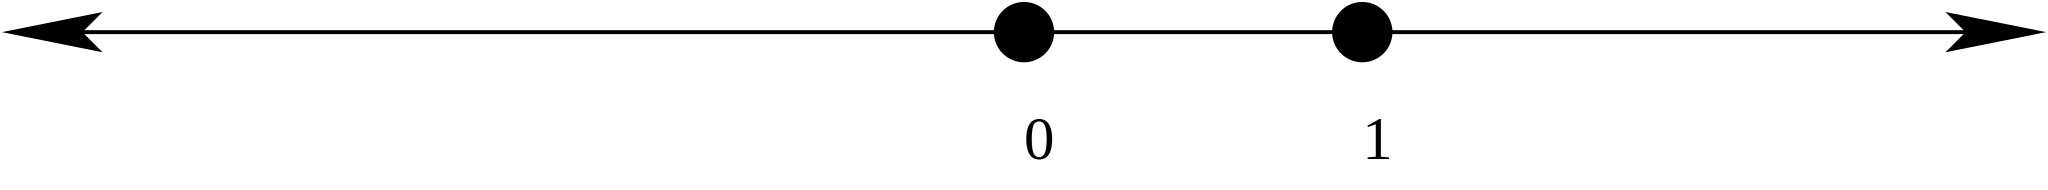
\includegraphics{../graphics/numberline.pdf}
\]
Label the left point $0$ and the right point $1$. If we think of this
as a starting point for a number line, then a \textbf{constructible
  number} is nothing more than a point we can obtain on the above
number line using one of the construction techniques above starting
with the points $0$ and $1$.  
\begin{enumerate}
\item Denote the set of numbers constructible by compass and
  straightedge with $\C$.\index{C@$\C$}\index{constructible numbers}
  We'll call $\C$ the set of \textit{constructible numbers}. 
\item Denote the set of numbers constructible by folding and tracing with
  $\F$.\index{F@$\F$}\index{folding and tracing numbers} We'll call $\F$ the set
  of \textit{folding and tracing numbers}.
\item Denote the set of numbers constructible by coordinate
  constructions with $\D$.\index{D@$\D$}\index{Descartes numbers} We'll
  call $\D$ the set of \textit{Descartes numbers}\marginnote{Be warned,
    this notion of so-called ``Descartes numbers'' is unique to these
    pages.}.
\end{enumerate}
Mostly in this chapter we'll be talking about $\C$. You'll have to
deal with $\F$ and $\D$ yourself.

\begin{question} Exactly what numbers are in $\C$?
\end{question}
\QM\index{set theory symbols!in@$\in$}\index{e@$\in$}

How do we attack this question?  Well first let's get a bit of
notation. Recall that we use the symbol ``$\in$'' to mean \textit{is
  in}. So we know that $0$ and $1$ are \textit{in} the set of
constructible numbers. So we write
\[
0\in \C \qquad\text{and}\qquad 1\in\C.
\]

\begin{question}
Is this true for $\F$, the set of folding and tracing numbers? What about
$\D$, the set of Descartes numbers?
\end{question}
\QM

If we could use constructions to make the operations $+$, $-$, $\cdot$, and $\div$, then we would be able to say a lot more.  In fact we will  do just this. 

\begin{question} 
How does one add and subtract using a compass and straightedge?
\end{question} 
\QM

\begin{question} 
Starting with $0$ and $1$, what numbers could we add to our number
line by simply adding and subtracting?
\end{question}

At this point we have all the positive whole numbers, zero, and the
negative whole numbers. We have a special name for this set, we call
it the \textbf{integers}\index{integers} and denote it by the letter
$\Z$:
\[
\Z = \{\dots, -5, -4, -3, -2, -1, 0, 1,2,3,4,5,\dots \}. \index{Z@$\Z$}
\]
\begin{question}
Are the integers contained in $\F$, the set of folding and tracing numbers? Are
the integers contained in $\D$, the set of Descartes numbers?
\end{question}
\QM

We still have some more operations:

\begin{construction}[Multiplication]\index{compass and straightedge!multiplication}\index{similar triangles} 
This construction is based on the idea of similar triangles. Start
with given segments of length $a$, $b$, and $1$:
\begin{enumerate}
 \item Make a small triangle with the segment  of length $1$ and segment of length $b$.
 \item Now place the segment of length $a$ on top of the unit segment  with one end at the vertex.
 \item Draw a line parallel to the segment connecting the unit to the segment of length $b$ starting at the other end of segment of length $a$.
 \item The length from the vertex to the point that the line containing $b$ intersects the line drawn in Step $3$ is of length $a\cdot b$.
\end{enumerate}
\[
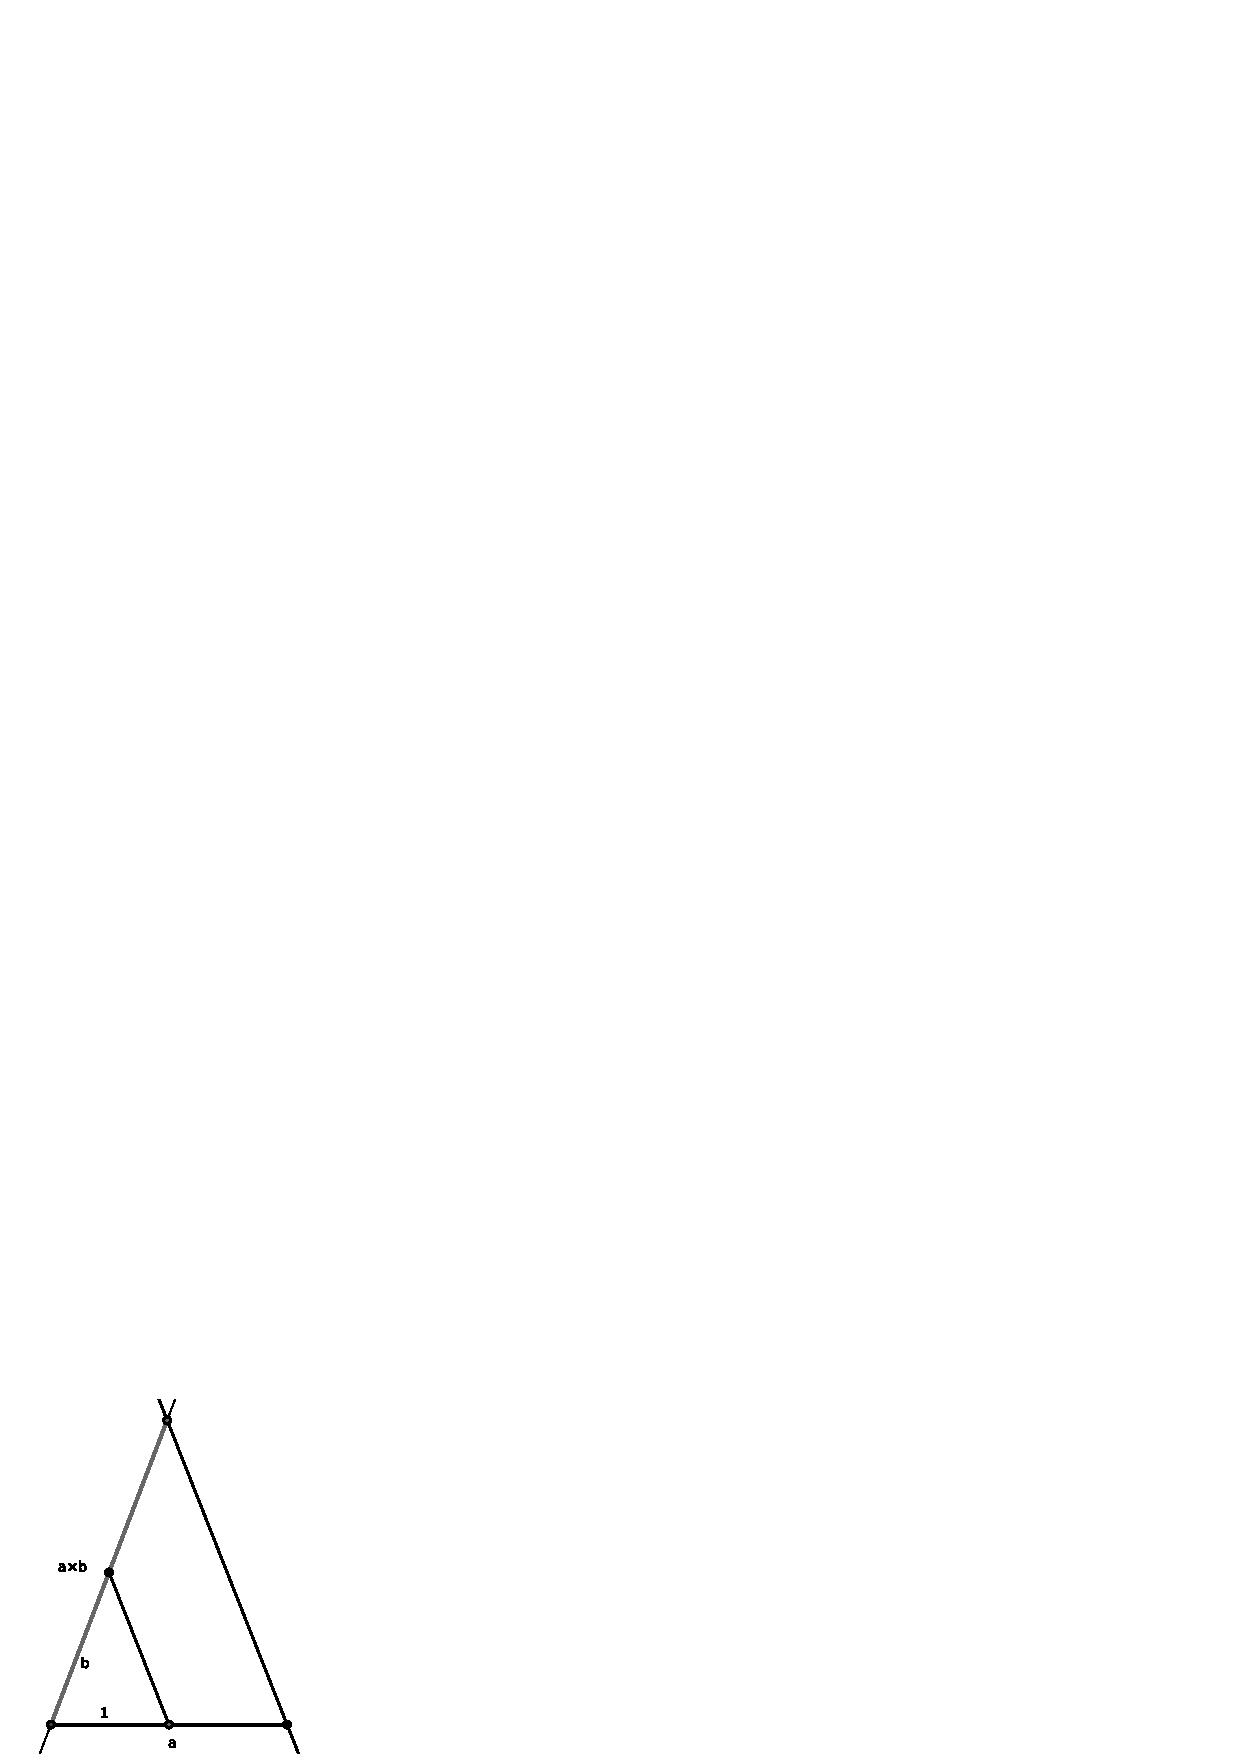
\includegraphics{../graphics/multiplication.pdf}
\]
\end{construction}
 

\begin{construction}[Division]\index{compass and straightedge!division}\index{similar triangles} 
This construction is also based on the idea of similar triangles.
Again, you start with given segments of length $a$, $b$, and $1$:
\begin{enumerate}
\item Make a triangle with  the segment of length $a$ and the segment of length $b$.
\item Put the unit along the segment of length $a$ starting at the vertex where the segment of length $a$ and the segment of length $b$ meet.
\item Make a line parallel to the third side of the triangle containing the segment of length $a$ and the segment of length $b$ starting at the end of the unit.
\item The distance from where the line drawn in Step $3$ meets the segment of length $b$ to the vertex is of length $b/a$.
\end{enumerate}
\[
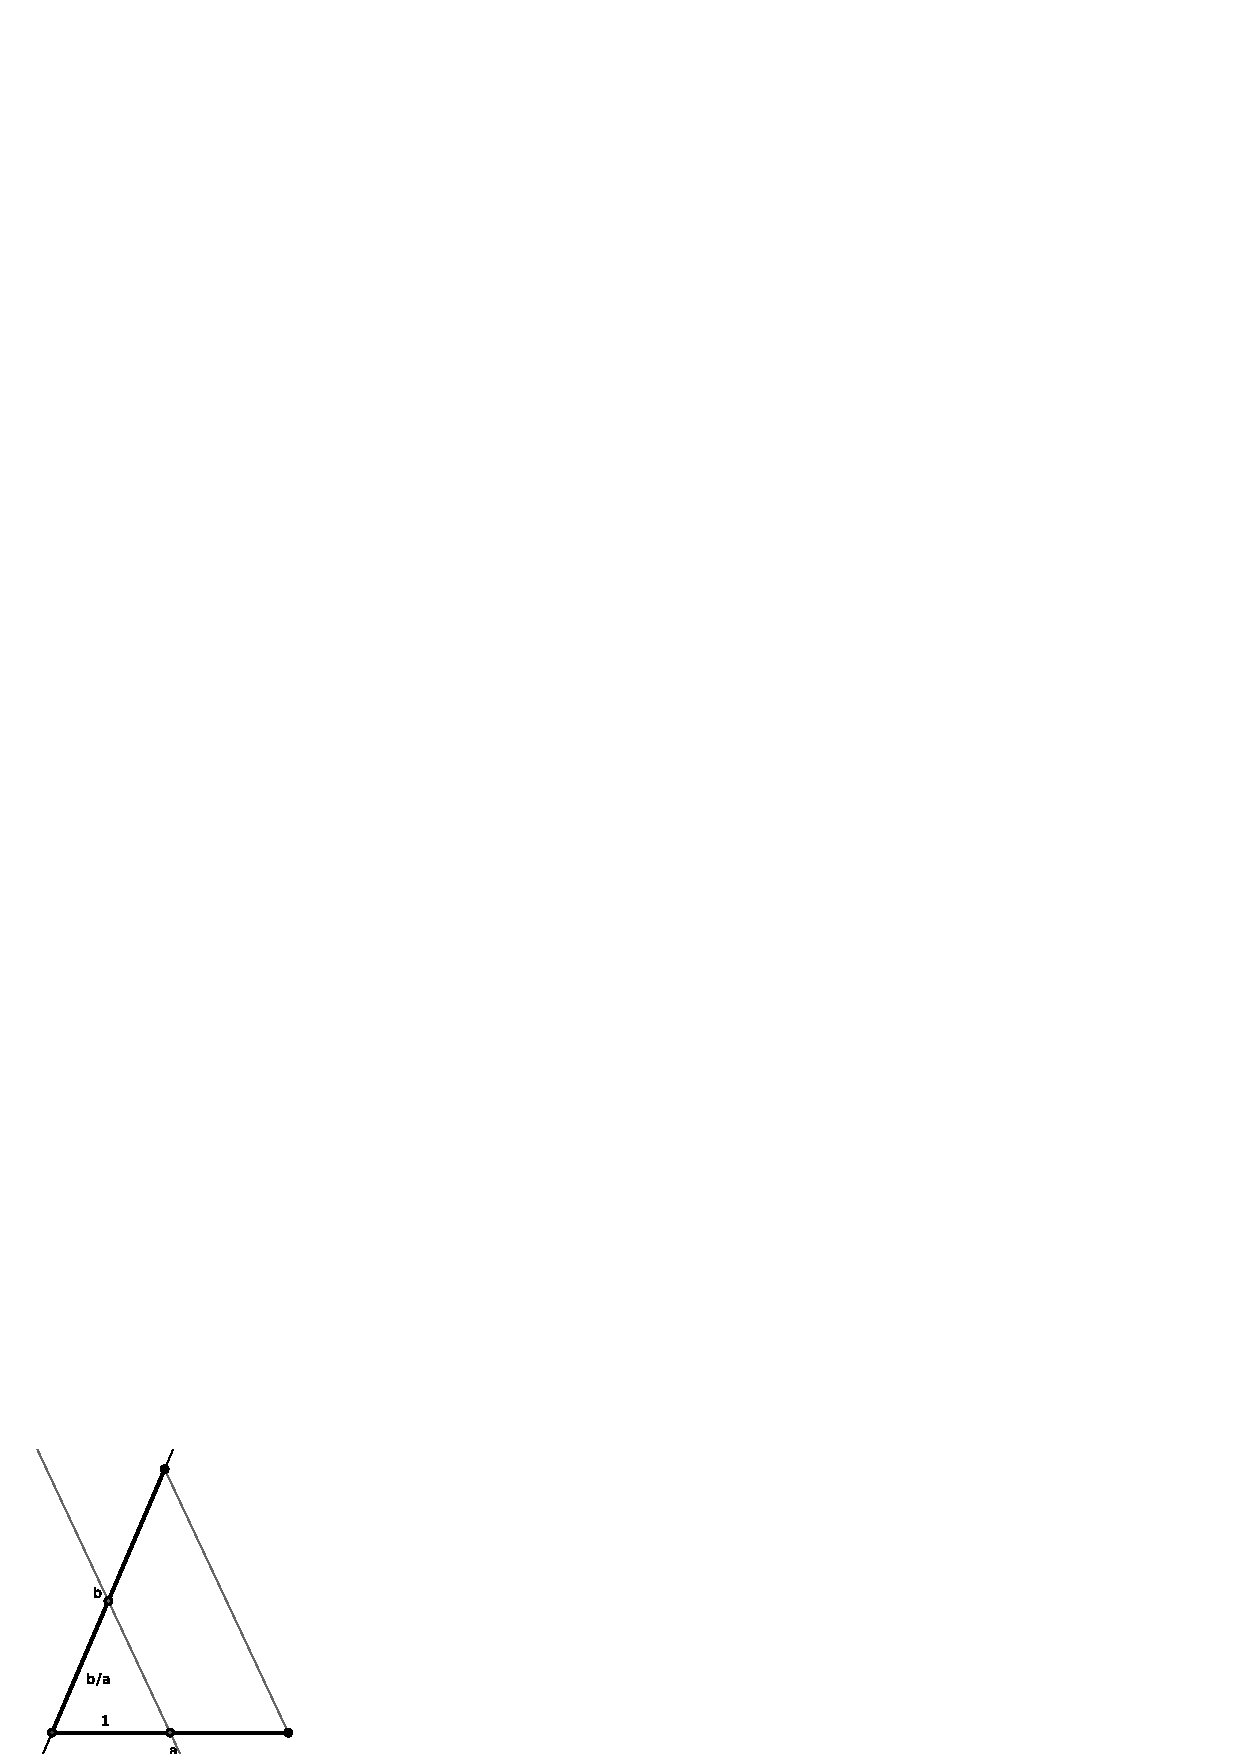
\includegraphics{../graphics/division.pdf}
\]
\end{construction}
 
\begin{question}
What does our number line look like at this point?
\end{question}
 

Currently we have $\Z$, the integers, and all of the fractions. In other words:
\[
      \Q = \left\{\frac{a}{b}\text{ such that $a\in\Z$ and $b\in\Z$ with $b\ne 0$}\right\}\index{Q@$\Q$}
\]
Fancy folks will replace the words \textit{such that} with a colon ``:'' to get:
\[
 \Q = \left\{\frac{a}{b}:\text{$a\in\Z$ and $b\in\Z$ with $b\ne 0$}\right\}
\]
We call this set the \index{rational numbers}\textbf{rational numbers}.  The letter $\Q$ stands for the word \textit{quotient}, which should remind us of fractions.


In mathematics we study sets of numbers. In any field of science, the first step to understanding something is to classify it. One sort of classification that we have is the notion of a \textit{field}.

\begin{definition}\index{field} A \textbf{field} is a set of numbers, which we will call $F$, that is closed under two associative and commutative operations $+$ and $\cdot$ such that:
\begin{enumerate}
\item 
\begin{enumerate} 
\item There exists an additive identity $0\in F$ such that for all $x\in F$, 
\[
x+0=x.
\]
\item For all $x\in F$, there is an additive inverse $-x\in F$ such that 
\[
x+ (-x) =0.
\]
\end{enumerate}
\item \begin{enumerate}
\item There exists a multiplicative identity $1\in F$ such that for all $x\in F$, 
\[
x\cdot 1 =x.
\]
\item For all $x\in F$ where $x\ne  0$, there is a multiplicative inverse $x^{-1}$  such that 
\[
x\cdot x^{-1}= 1.
\]
\end{enumerate}
\item Multiplication distributes over addition. That is, for all $x,y,z\in F$
\[
x\cdot (y+z)=x\cdot y+x\cdot z.
\]
\end{enumerate}
\end{definition}

Now, a word is in order about three tricky words I threw in above: \textit{closed}, \textit{associative}, and \textit{commutative}: 

\begin{definition}\index{closed} A set $F$ is \textbf{closed} under an operation $\star$ if for all $x,y\in F$, $x\star y\in F$.   
\end{definition}

\begin{example} The set of integers, $\Z$, is closed under addition, but is not closed under division.
\end{example}

\begin{definition}\index{associative} An operation $\star$ is \textbf{associative} if for all $x$, $y$, and $z$
\[
x\star(y \star z) = (x \star y) \star z.
\]   
\end{definition}

\begin{definition}\index{commutative} An operation $\star$ is \textbf{commutative} if for all $x$, $y$
\[
x\star y  =  y \star x.
\]   
\end{definition}


\begin{question} Is $\Z$ a field?  Is $\Q$ a field?  Can you think of other fields?  What about the set of constructible numbers $\C$? What about the folding and tracing numbers $\F$? What about the Descartes numbers $\D$?
\end{question}
\QM

From all the constructions above we see that the set of constructible
numbers $\C$ is a field. However, which field is it? In fact, the set
of constructible numbers is bigger than $\Q$!

\begin{construction}[Square-Roots] Start with given segments of length $a$ and $1$:
\begin{enumerate}
\item  Put the segment of length $a$ immediately to the left of 
the unit segment on a line. 
\item Bisect the segment of length $a + 1$.
\item Draw an arc centered at the bisector that starts at one 
end of the line segment of length $a + 1$ and ends at the other end. 
\item Construct the perpendicular at the point where the segment of length $a$ meets the unit. 
\item The line segment connecting the meeting point of the segment of length $a$ and the unit to the arc drawn in Step $3$ is of length $\sqrt{a}$. 
\end{enumerate}
\[
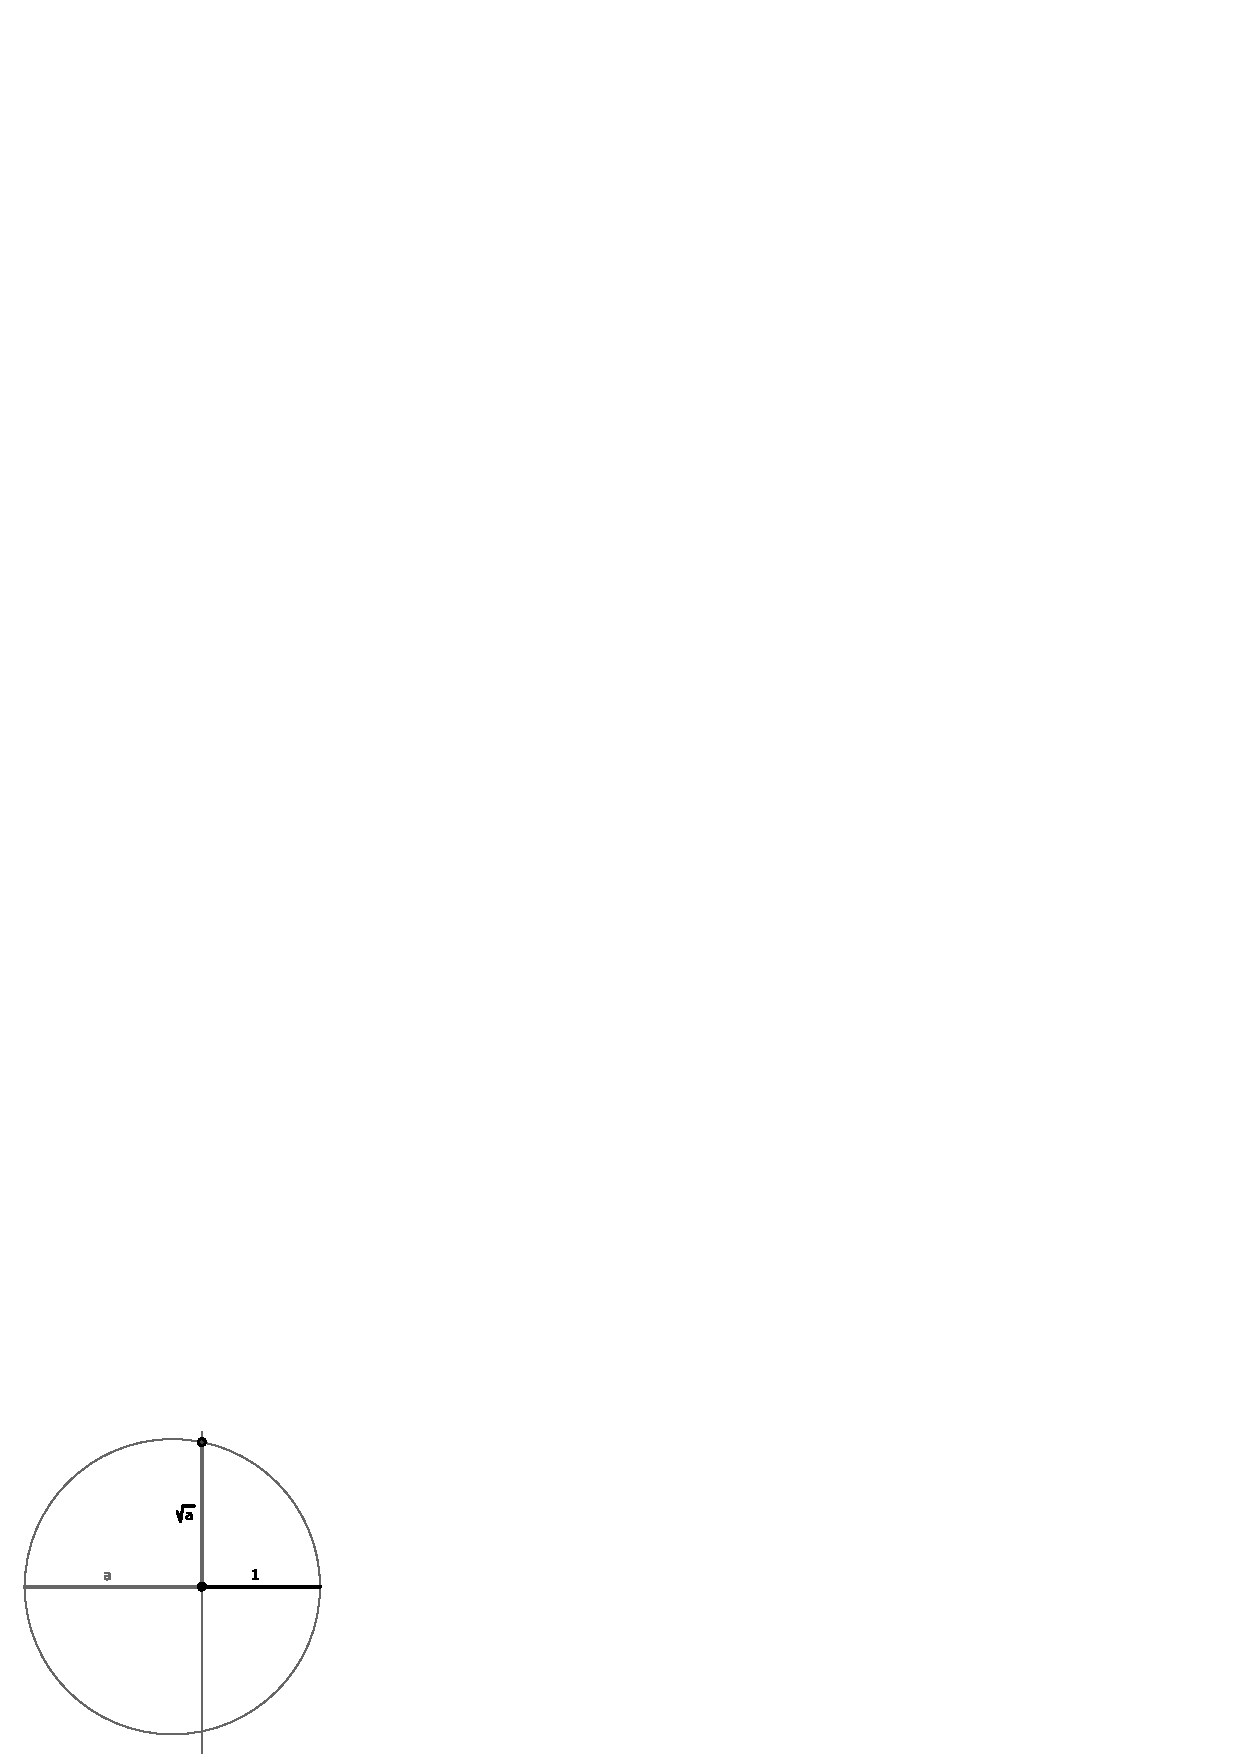
\includegraphics{../graphics/sqrt.pdf}
\]
\end{construction}

This tells us that square-roots are constructible. In particular, the square-root of two is constructible. But the square-root of two is not rational! That is, there is no fraction
\[
\frac{a}{b} = \sqrt{2} \qquad \text{such that $a,b\in\Z$}.
\]

\begin{question} 
Can you remind me, how do we know that $\sqrt{2}$ is not rational?
\end{question}
\QM

\begin{question} 
Are square-roots found in $\F$, the set of folding and tracing numbers? What about
$\D$, the set of Descartes numbers?
\end{question}
\QM

OK, so how do we talk about a field that contains both $\Q$ and
$\sqrt{2}$? Simple, use this notation:\index{Qalpha@$\Q(\alpha)$}
\[
\Q(\sqrt{2})= \{\text{the smallest field containing both $\Q$ and $\sqrt{2}$}\}
\]
So the set of constructible numbers contains all of $\Q( \sqrt{2} )$. Does the set of constructible numbers contain even more numbers? Yes! In fact the $\sqrt{3}$ is also not rational, but is constructible. So here is our situation:
\[
\Z \subset \Q \subset \Q(\sqrt{2}) \subset \Q(\sqrt{2},\sqrt{3}) \subset \C
\]

So all the numbers in $\Q(\sqrt{2},\sqrt{3})$ are also in $\C$. But is
this all of $\C$? Hardly! We could keep on going, adding more and more
square-roots 'til the cows come home, and we still will not have our
hands on all of the constructible numbers. But all is not lost. We can
still say something:


\begin{theorem} 
The use of compass and straightedge alone on a field $F$ can at most
produce numbers in a field $F( \sqrt{\alpha} )$ where $\alpha \in F$.
\end{theorem}

\begin{question} Can you explain why the above theorem is true? Big hint: What is the relationship between $\C$ and $\D$?
\end{question}
\QM


The upshot of the above theorem is that the only numbers that are
constructible are expressible as a combination of rational numbers and
the symbols:
\[
+\quad -\quad \cdot\quad \div \quad \sqrt{\hspace{1em}}
\]

So what are examples of numbers that are not constructible? Well to
start $\sqrt[3]{2}$ is not constructible. Also $\pi$ is not
constructible. While both of these facts can be carefully explained,
we will spare you gentle reader---for now\marginnote{The most accessible
  discussion of this fact that I know of can be found in
  \cite{coruant}.}.

\begin{question} Which of the following numbers are constructible?
\[
3.1415926, \qquad \sqrt[16]{5}, \qquad \sqrt[3]{27}, \qquad \sqrt[6]{27}.
\]
\end{question}
\QM



\begin{problems}
\begin{enumerate}
\item Explain what the set denoted by $\Z$ is.
\item Explain what the set denoted by $\Q$ is.
\item Explain what the set $\C$ of constructible numbers is.
\item Given two line segments $a$ and $b$, construct $a+b$. Explain
  the steps in your construction.
\item Given two line segments $a$ and $b$, construct $a-b$. Explain
  the steps in your construction.
\item Given three line segments $1$, $a$, and $b$, construct $a\cdot
  b$. Explain the steps in your construction.
\item Given three line segments $1$, $a$, and $b$, construct
  $a/b$. Explain the steps in your construction.
\item Given a unit, construct $4/3$. Explain the steps in your
  construction.
\item Given a unit, construct $3/4$. Explain the steps in your
  construction.
\item Use the construction for multiplication to explain why when
  multiplying two numbers between $0$ and $1$, the product is always
  still between $0$ and $1$.
\item Explain why the construction for multiplication works.
\item Use the construction for division to explain why when dividing a
  positive number by a number between $0$ and $1$, the quotient is
  always larger than the initial positive number.
\item Explain why the construction for division works.
\item Given a unit, construct $\sqrt{2}$. Explain the steps in your
  construction.
\item Use algebra to help explain why the construction for
  square-roots works.

\item Give relevant and revealing examples of numbers in the set $\Z$.
\item Give relevant and revealing examples of numbers in the set $\Q$.
\item Give relevant and revealing examples of numbers in the set
  $\Q(\sqrt{2})$.
\item Give relevant and revealing examples of numbers in the set
  $\Q(\sqrt{2},\sqrt{3})$.
\item Give relevant and revealing examples of numbers in the set
  $\Q(\sqrt{2},\sqrt{3},\sqrt{5})$.
\item Which of the following are constructible numbers? Explain your
  answers.
\begin{enumerate} 
\item $3.141$
\item $\sqrt[3]{5}$
\item $\sqrt{3 + \sqrt{17}}$
\item $\sqrt[8]{5}$
\item $\sqrt[10]{37}$
\item $\sqrt[16]{37}$
\item $\sqrt[3]{28}$
\item $\sqrt[3]{27}$
\item $\sqrt{13+\sqrt[3]{2} + \sqrt{11}}$
\item $3+ \sqrt[5]{4}$
\item $\sqrt{3+\sqrt{19} + \sqrt{10}}$
\end{enumerate}
\item Is $\sqrt{7}$ a rational number? Is it a constructible number?
  Explain your reasoning.
\item Is $\sqrt{8}$ a rational number? Is it a constructible number?
  Explain your reasoning.
\item Is $\sqrt{9}$ a rational number? Is it a constructible number?
  Explain your reasoning.
\item Is $\sqrt[3]{7}$ a rational number? Is it a constructible
  number? Explain your reasoning.
\item Is $\sqrt[3]{8}$ a rational number? Is it a constructible
  number? Explain your reasoning.
\item Is $\sqrt[3]{9}$ a rational number? Is it a constructible
  number? Explain your reasoning.
\end{enumerate}
\end{problems}

\newpage


\section{Impossibilities}\index{compass and straightedge!impossible problems}

Oddly enough, the importance of compass and straightedge 
constructions is not so much what we can construct, but what 
we cannot construct. It turns out that classifying what we cannot construct is an interesting question.  There are three classic problems which are 
impossible to solve with a compass and straightedge alone:
\begin{enumerate}
\item Doubling the cube.
\item Squaring the circle.
\item Trisecting the angle.
\end{enumerate}

\subsection{Doubling the Cube}\index{doubling the cube}

The goal of this problem is to double the volume of a given cube.  
This boils down to trying to construct roots to the equation:
\[
x^3-2=0
\]
But we can see that the only root of the above equation is $\sqrt[3]{2}$ and  we already know that this number is not constructible.  

\begin{question} Why does doubling the cube boil down to constructing a solution to the equation $x^3-2=0$?
\end{question}
\QM

\subsection{Squaring the Circle}\index{squaring the circle}  
Given a circle of radius $r$, we wish to 
construct a square that has the same area. Why would someone want to do such a thing? Well to answer this question you must ask yourself:

\begin{question} What is area?
\end{question}
\QM

So what is the deal with this problem? Well suppose you have a circle of radius 1. Its area is now $\pi$ square units. How long should the edge of a square be if it has the same area? Well the square should have sides of length $\sqrt{\pi}$ units. In 1882, it was proved that $\pi$ is not the root of any polynomial equation, and hence $\sqrt{\pi}$ is not constructible. Therefore, it is impossible to square the circle.



\subsection{Trisecting the Angle}\index{trisecting the angle}
This might sound like the easiest to understand, but it's a bit
subtle.  Given any angle, the goal is to trisect that angle.  It can
be shown that this cannot be done using a compass and straightedge. In
particular, it is impossible to trisect a $60$ degree angle with
compass and straightedge alone.  However, we are not saying that you
cannot trisect some angles with compass and straightedge alone, in
fact there are \textit{special} angles which can be trisected using a
compass and straightedge. However the methods used to trisect those
special angles will fail miserably in nearly all other cases.

\begin{question} Can you think of any angles that can be trisected 
using a compass and straightedge?
\end{question}
\QM

Just because it is impossible to trisect an arbitrary angle with
compass and straightedge alone does not stop people from trying.

\begin{question} 
If you did not know that it was impossible to trisect an arbitrary
angle with a compass and straightedge alone, how might you try to do
it?
\end{question}
\QM


One common way that people try to trisect angles is to take an angle,
make an isosceles triangle using the angle, and divide the line segment
opposite the angle into three equal parts. While you can divide the
opposite side into three equal parts, it in fact \textbf{never}
trisects the angle. When you do this procedure to acute angles, it
\emph{seems} to work, though it doesn't really. You can see that it
doesn't by looking at an obtuse angle:
\[
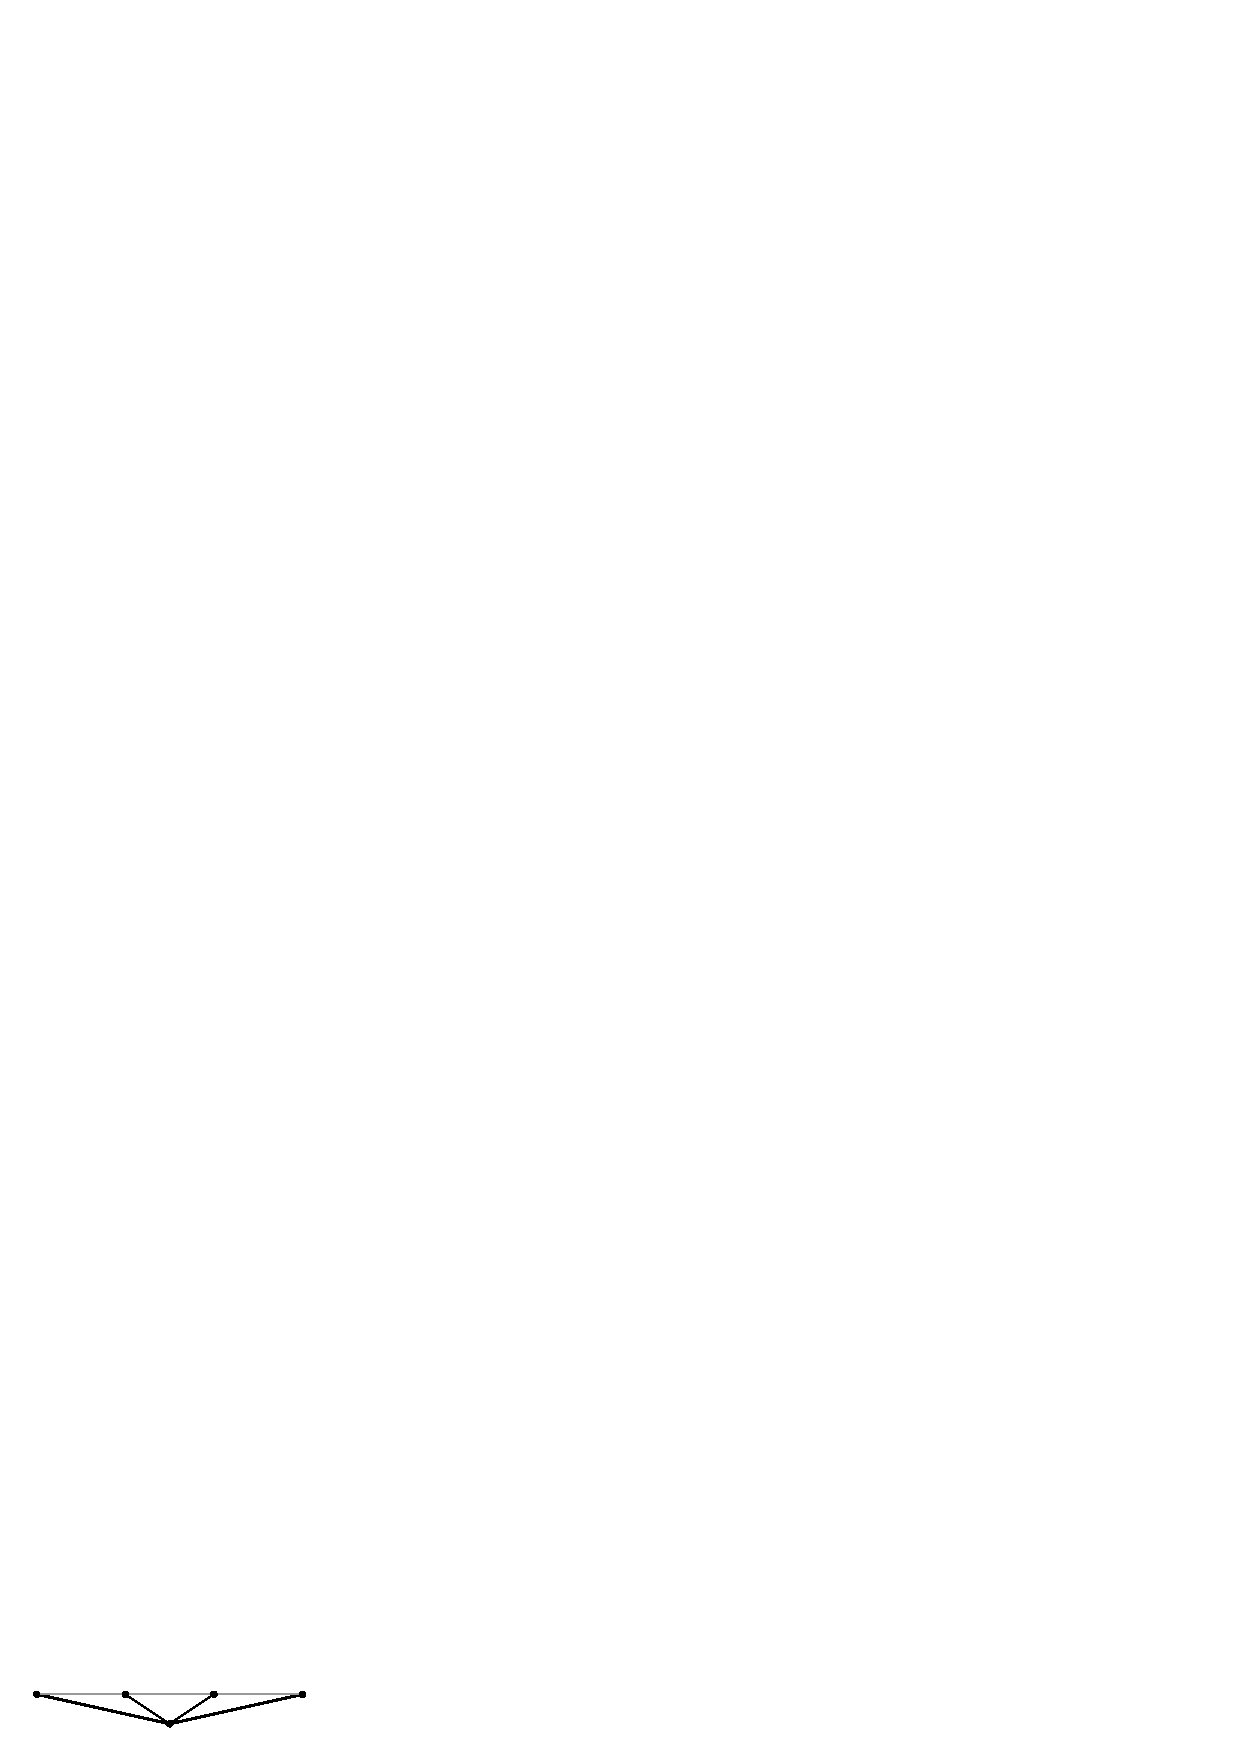
\includegraphics{../graphics/impostrisect.pdf}
\]
Trisecting the line segment opposite the angle clearly leaves the
middle angle much larger than the outer two angles. This happens
regardless of the measure of the angle. This mistake is common among
people who think that they can trisect an angle with compass and
straightedge alone.

\subsection{Folding and Tracing's Time to Shine}

We know that:
\[
\Z \subset \Q \subset \Q(\sqrt{2}) \subset \Q(\sqrt{2},\sqrt{3}) \subset \C = \D
\]
Where does the set of folding and tracing numbers $\F$ fit into the parade? I'll
tell you, if you promise not to tell anybody that I did\dots $\F$ is
the leader of the pack! We already know that you can trisect angles
using folding and tracing constructions. In fact you can even solve cubic
equations! We'll show you how to do this.

\begin{construction}[Solving Cubic Equations]\index{folding and tracing!solving cubic equations}\index{cubic equations!folding and tracing} We wish to solve equations of the form:
\[
x^3 + ax^2 + bx + c = 0
\]
\begin{enumerate}
\item Plot the points: $P_1 = (a,1)$ and $P_2 = (c,b)$.
\item Plot the lines: $\l_1: y = -1$ and $\l_2: x= -c$.
\item With a single fold, place $P_1$ onto $\l_1$ and $P_2$ onto $\l_2$.
\item The slope of the crease is a solution to $x^3 + ax^2 + bx + c =
  0$.
\end{enumerate}
\[
\includegraphics{../graphics/origamiCube.pdf}
\]
\end{construction}

\begin{question} How do we get the ``solution'' from the slope?
\end{question}
\QM

Since folding and tracing constructions can duplicate every compass and
straightedge construction and more, we have that $\C \subset \F$.


\begin{problems}
\begin{enumerate}
\item Explain the three classic problems that cannot be solved with a
  compass and straightedge alone.
\item Use a compass and straightedge construction to trisect an angle
  of $90^\circ$. Explain the steps in your construction.
\item Use a compass and straightedge construction to trisect an angle
  of $135^\circ$. Explain the steps in your construction.
\item Use a compass and straightedge construction to trisect an angle
  of $45^\circ$. Explain the steps in your construction.
\item Use a compass and straightedge construction to trisect an angle
  of $67.5^\circ$. Explain the steps in your construction.
\item Use folding and tracing to construct an angle of $20^\circ$. Explain the
  steps in your construction.
\item Use folding and tracing to construct an angle of $10^\circ$. Explain the
  steps in your construction.
\item Is it possible to use compass and straightedge constructions to
  construct an angle of $10^\circ$? Why or why not?
\item We have seen that:
\[
\Z \subset \Q \subset \Q(\sqrt{2}) \subset \Q(\sqrt{2},\sqrt{3})
\subset \C \subset \F
\]
Give explicit examples showing that the set inclusions above are
strict---none of them are set equality. Explain your reasoning.
\item Use folding and tracing to find a solution to the following cubic equations:
\begin{enumerate}
\item $x^3-x^2 -x+1= 0$ 
\item $x^3-2x^2 -x + 2 = 0$ 
\item $x^3 -3x-2=0$
\item $x^3-4x^2 +5x-2=0$
\item $x^3-2x^2-5x+6=0$
\end{enumerate}
Explain the steps in your constructions.
\end{enumerate}
\end{problems}

